% This is text associated with the open textbook "Open Electromagnetics"
% See immediately below for author, date
% This work is licensed under the Creative Commons Attribution-ShareAlike 4.0 International License. (CC BY SA 4.0) 
% To view a copy of the license, visit http://creativecommons.org/licenses/by-sa/4.0/

%ORB TITLE Complex Permittivity
%ORB AUTHOR 0        # S.W. Ellingson, Virginia Tech (ellingson@vt.edu)
%ORB DATE 20191212   # yyyymmdd
%ORB ABSTRACT  

\label{m0134_Complex_Permittivity} % <-- Must match name of this file and module directory name.  Don't mess with this!
\index{permittivity!complex-valued|(}

The relationship between 
electric field intensity ${\bf E}$ (SI base units of V/m)
and 
electric flux density ${\bf D}$ (SI base units of C/m$^2$)
is:
%
\begin{equation}
{\bf D} = \epsilon{\bf E}
\label{m0134_eD}
\end{equation}
%
where 
$\epsilon$ is the permittivity (SI base units of F/m).
In simple media, $\epsilon$ is a real positive value which does not depend on the time variation of ${\bf E}$.
That is, the response (${\bf D}$) to a change in ${\bf E}$ is observed instantaneously and without delay.

In practical materials, however, the change in ${\bf D}$ in response to a change in ${\bf E}$ may depend on the manner in which ${\bf E}$ changes.
The response may not be instantaneous, but rather might take some time to fully manifest. 
This behavior can be modeled using the following generalization of Equation~\ref{m0134_eD}:
%
\begin{equation}
{\bf D} = a_0{\bf E} + a_1 \frac{\partial}{\partial t} {\bf E} + a_2 \frac{\partial^2}{\partial t^2} {\bf E} + a_3 \frac{\partial^3}{\partial t^3} {\bf E} + ...
\label{m0134_ee}
\end{equation}
%
where $a_0$, $a_1$, $a_2$, and so on are real-valued constants, and the number of terms is infinite.
In practical materials, the importance of the terms tends to diminish with increasing order.
Thus, it is common that only the first few terms are significant. 
In many applications involving common materials, only the first term is significant; i.e., $a_0\approx\epsilon$ and $a_n\approx 0$ for $n\ge 1$.
As we shall see in a moment, this distinction commonly depends on frequency.  

In the phasor domain, differentiation with respect to time becomes multiplication by $j\omega$.
Thus, Equation~\ref{m0134_ee} becomes
%
\begin{flalign} 
\widetilde{\bf D} &= a_0\widetilde{\bf E} + a_1\left(j\omega\right)\widetilde{\bf E} + a_2\left(j\omega\right)^2\widetilde{\bf E} + a_3\left(j\omega\right)^3\widetilde{\bf E} + ... \nonumber \\
                  &= a_0\widetilde{\bf E} + j\omega a_1\widetilde{\bf E} - \omega^2 a_2\widetilde{\bf E} - j\omega^3 a_3\widetilde{\bf E} + ... \nonumber \\
                  &= \left(a_0 + j\omega a_1 - \omega^2 a_2 - j\omega^3 a_3 + ... \right) \widetilde{\bf E} 
\end{flalign}
%
Note that the factor in parentheses is a complex-valued number which depends on frequency $\omega$ and materials parameters $a_0$, $a_1$, ...
We may summarize this as follows:
%
\begin{equation} 
\widetilde{\bf D} = \epsilon_c \widetilde{\bf E} 
\label{m0134_eDc}
\end{equation}
%
where $\epsilon_c$ is a complex-valued constant that depends on frequency.
\index{permittivity!complex-valued}

The notation ``$\epsilon_c$'' is used elsewhere in this book (e.g., Section~\ref{m0128_Wave_Equations_Lossy_Regions}) to represent a generalization of simple permittivity that accommodates loss associated with non-zero conductivity $\sigma$.
In Section~\ref{m0128_Wave_Equations_Lossy_Regions}, we defined
%
\begin{equation}
\epsilon_c \triangleq \epsilon' -j\epsilon'' 
\end{equation}
where 
$\epsilon' \triangleq \epsilon$ (i.e., real-valued, simple permittivity) and
$\epsilon'' \triangleq \sigma/\omega$ (i.e., the effect of non-zero conductivity). 
Similarly, $\epsilon_c$ in Equation~\ref{m0134_eDc} can be expressed as
%
\begin{equation}
\epsilon_c \triangleq \epsilon' -j\epsilon'' 
\end{equation}
%
but in this case 
%
\begin{equation}
\epsilon' \triangleq a_0 - \omega^2a_2 + ...
\end{equation}
% 
and
%
\begin{equation}
\epsilon'' \triangleq -\omega a_1 + \omega^3a_3 - ... 
\end{equation}

%%%%%%%%%%%%%%%%%%%%%%%%%%%%%%%%%%%%%%%%%%%%%%%
%ORB HIGHLIGHT
\begin{mdframed}[backgroundcolor=yellow!20,nobreak=true] 
When expressed as phasors, the temporal relationship between electric flux density and electric field intensity can be expressed as a complex-valued permittivity.
\end{mdframed}
%%%%%%%%%%%%%%%%%%%%%%%%%%%%%%%%%%%%%%%%%%%%%%%

Thus, we now see two possible applications for the concept of complex permittivity:
Modeling the delayed response of ${\bf D}$ to changing ${\bf E}$, as described above; and
modeling loss associated with non-zero conductivity.
In practical work, it may not always be clear precisely what combination of effects the complex permittivity $\epsilon_c = \epsilon'-j\epsilon''$ is taking into account.
For example, if $\epsilon_c$ is obtained by measurement, both delayed response and conduction loss may be represented.
Therefore, it is not reasonable to assume a value of $\epsilon''$ obtained by measurement represents only conduction loss (i.e., is equal to $\sigma/\omega$); in fact, the measurement also may include a significant frequency-dependent contribution associated with the delayed response behavior identified in this section.

An example of the complex permittivity of a typical dielectric material is shown in Figure~\ref{m0134_fDielectric_responses}.
Note the frequency dependence is quite simple and slowly-varying at frequencies below 1~GHz or so, but becomes relatively complex at higher frequencies.
%
\begin{figure} %[b!]
\begin{center}
\pdftooltip{{  % note double braces
%\vspace{3in} 
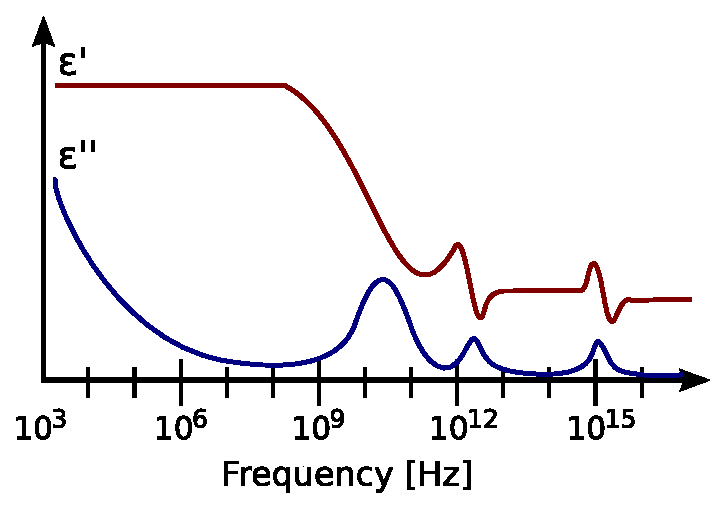
\includegraphics[width=\columnwidth]{modules/m0134_Dielectric_responses.eps} 
% https://commons.wikimedia.org/wiki/File:Dielectric_responses.svg
}}{x-y plot of permittivity versus frequency in hertz. X-axis scale is from 10 power 3 to ten power 16 with increments of powers of 10. There are two curves plotted, small epsilon prime and small epsilon double prime. Small epsilon prime is always above small epsilon double prime.}
\end{center}
\centerline{\scriptsize 
\copyright~\hyperref[m0134_Dielectric_responses_credit]{K.A.\ Mauritz (modified)} 
} 
\caption{
\label{m0134_fDielectric_responses}
The relative contributions of the real and imaginary components of permittivity for a typical dielectric material (in this case, a polymer).
}
\end{figure}

~\\
%%%%%%%%%%%%%%%%%%%%%%%%%%%%%%%%%%%%%%%%%%%%%%%%%%%%%%%

{\bf Additional Reading:}
\begin{itemize}
\item ``\href{https://en.wikipedia.org/wiki/Permittivity}{Permittivity}'' on Wikipedia.
\end{itemize}


\index{permittivity!complex-valued|)}
